\chapter{Lípidos}\label{ch:b1:lipids}

Un camello que cruza un desierto lleva treinta kilogramos de \omterm{def:b1:lipids:triglyceride}{grasa} en su
joroba y allí ni una gota de agua; una trucha de un arroyo de montaña a
\qty{4}{\celsius} tiene membranas tan fluidas como las de una carpa en un
estanque templado; y una gota de \omterm{def:b1:lipids:triglyceride}{aceite} de oliva agitada en agua se rompe en
una nube de gotitas que, si se las deja, vuelven a reunirse en una sola. Los
tres son \omterm{def:b1:lipids:fattyacid}{lípidos} en acción: la reserva más densa de energía química que un
\omterm{def:b1:organism-environment:organism}{organismo} puede llevar, la película que limita cada \omterm{def:b1:cell-unit-of-life:cell}{célula} y cada orgánulo,
y la clase de molécula que el agua se niega a disolver. Este capítulo
describe los \omterm{def:b1:lipids:fattyacid}{ácidos grasos} y las \omterm{def:b1:lipids:triglyceride}{grasas} construidas con ellos, los \omterm{def:b1:lipids:fattyacid}{lípidos}
\omterm{def:b1:lipids:amphiphilic}{anfífilos} que se ensamblan en membranas, lo que hace a una membrana más o
menos fluida, y los demás \omterm{def:b1:lipids:fattyacid}{lípidos} --- \omterm{def:b1:lipids:amphiphilic}{esteroles}, pigmentos, hormonas --- que
unos pocos carbonos dispuestos en anillos y cadenas pueden llegar a ser.

\section{Ácidos grasos}

\begin{definition}[Lípido, ácido graso]\label{def:b1:lipids:fattyacid}
Los \emph{lípidos}\index{lípido} son las moléculas biológicas definidas no
por una estructura común, sino por una propiedad común: son insolubles en
agua y solubles en disolventes apolares. Casi todos están construidos sobre
\emph{ácidos grasos}\index{ácido graso}: ácidos carboxílicos con una cadena
hidrocarbonada sin ramificar de \qtyrange{12}{24}{} carbonos, casi siempre
en número par (se ensamblan de dos en dos carbonos,
\cref{ch:b1:biosyntheses-integration}). Un ácido graso
\emph{saturado}\index{ácido graso saturado} solo tiene enlaces sencillos y
una cadena recta y flexible; uno \emph{insaturado}\index{ácido graso insaturado} tiene uno o más enlaces dobles, en configuración \emph{cis},
cada uno de los cuales introduce en la cadena un codo rígido de unos
$30^\circ$. Notación: C18:1 $\Delta^9$ es un ácido de 18 carbonos con un
enlace doble tras el carbono 9 (ácido oleico); un ácido \emph{omega-3} tiene
su último enlace doble a tres carbonos del extremo metilo.
\end{definition}

\begin{omfigure}
\begin{tikzpicture}[font=\footnotesize, line cap=round, line join=round]
  % stearic acid: zig-zag of 18 carbons
  \draw[very thick, omDef!80!black] (0,0) \foreach \i in {1,...,17} { -- ++({0.36}, {0.22*(-1)^\i}) };
  \node[fill=omThm!25, draw=omThm, rounded corners=2pt, inner sep=2pt] at (-0.1,0.0) {COOH};
  \node[anchor=east, align=right] at (-0.85,0) {ácido esteárico C18:0\\ saturado, recto\\ funde a \qty{70}{\celsius}};
  \node[anchor=west] at (6.3,-0.22) {$\mathrm{CH_3}$};
  % oleic acid: kink at carbon 9-10, second half tilted downward
  \draw[very thick, omDef!80!black] (0,-2.0) \foreach \i in {1,...,8} { -- ++({0.36}, {0.22*(-1)^\i}) };
  \draw[very thick, omDef!80!black] (2.88,-2.0) -- ++(0.36,0.22);
  \draw[double, very thick, omThm] (3.24,-1.78) -- ++(0.36,0.22);
  \draw[very thick, omDef!80!black] (3.60,-1.56) \foreach \i in {1,...,8} { -- ++({0.33}, {0.22*(-1)^(\i+1)-0.13}) };
  \node[fill=omThm!25, draw=omThm, rounded corners=2pt, inner sep=2pt] at (-0.1,-2.0) {COOH};
  \node[anchor=east, align=right] at (-0.85,-2.0) {ácido oleico C18:1 $\Delta^9$\\ un doble enlace \emph{cis}, acodado\\ funde a \qty{13}{\celsius}};
  \node[omThm, anchor=south] at (3.42,-1.45) {doble enlace \emph{cis}};
  \node[anchor=west] at (6.35,-2.62) {$\mathrm{CH_3}$};
\end{tikzpicture}

{\small Dos \omterm{def:b1:lipids:fattyacid}{ácidos grasos} de 18 carbonos. La cadena saturada es recta y se
empaqueta estrechamente contra sus vecinas; el doble enlace \emph{cis} del
ácido oleico dobla la cadena y mantiene apartadas a las vecinas, y por eso
el ácido oleico es líquido a temperatura ambiente y el esteárico, sólido.}
\end{omfigure}

\begin{proposition}[Puntos de fusión]\label{prop:b1:lipids:melting}
El punto de fusión de un \omterm{def:b1:lipids:fattyacid}{ácido graso}, y la \omterm{def:b1:lipids:fluidity}{fluidez} de cualquier conjunto
lipídico al que pertenezca, lo fija lo estrechamente que puedan empaquetarse
las cadenas: sube con la longitud de la cadena (\qty{44}{\celsius} para
C12:0, \qty{63}{\celsius} para C16:0, \qty{70}{\celsius} para C18:0) y baja
bruscamente con cada doble enlace \emph{cis} (C18:0 \qty{70}{\celsius},
C18:1 \qty{13}{\celsius}, C18:2 \qty{-5}{\celsius}, C18:3
\qty{-11}{\celsius}). Las \omterm{def:b1:lipids:triglyceride}{grasas} animales, ricas en ácidos saturados, son
sólidas a temperatura ambiente; los \omterm{def:b1:lipids:triglyceride}{aceites} vegetales y de pescado, ricos en
\omterm{def:b1:lipids:fattyacid}{insaturados}, son líquidos.
\end{proposition}
\begin{proof}
Las cadenas rectas se colocan lado a lado y cada $\mathrm{CH_2}$ establece
contactos de \omterm{def:b1:water-small-molecules:bonds}{van der Waals} con sus vecinas, cada uno de unos pocos
kilojulios por mol, sumados a lo largo de la cadena: más carbonos, más
contactos, más calor para separarlas. Un codo impide el contacto estrecho a
lo largo de varios carbonos a cada lado y suprime muchos contactos de golpe.
\end{proof}

\section{Las grasas: la reserva de energía}

\begin{definition}[Triglicérido]\label{def:b1:lipids:triglyceride}
Un \emph{triglicérido}\index{triglicérido} (triacilglicerol, una
\emph{grasa}\index{grasa} cuando es sólido y un \emph{aceite}\index{aceite}
cuando es líquido) es glicerol --- un alcohol de tres carbonos ---
esterificado en sus tres hidroxilos por tres \omterm{def:b1:lipids:fattyacid}{ácidos grasos}. No tiene carga
ni le queda ningún grupo \omterm{def:b1:water-small-molecules:water}{polar}: es enteramente hidrófobo, y se almacena en
forma de gotas anhidras en los \emph{adipocitos}\index{adipocito}, \omterm{def:b1:cell-unit-of-life:cell}{células}
del \omterm{def:b1:body-plans-tissues:tissue}{tejido} adiposo que son poco más que una gota de grasa con el núcleo
desplazado a un lado.
\end{definition}

\begin{omfigure}
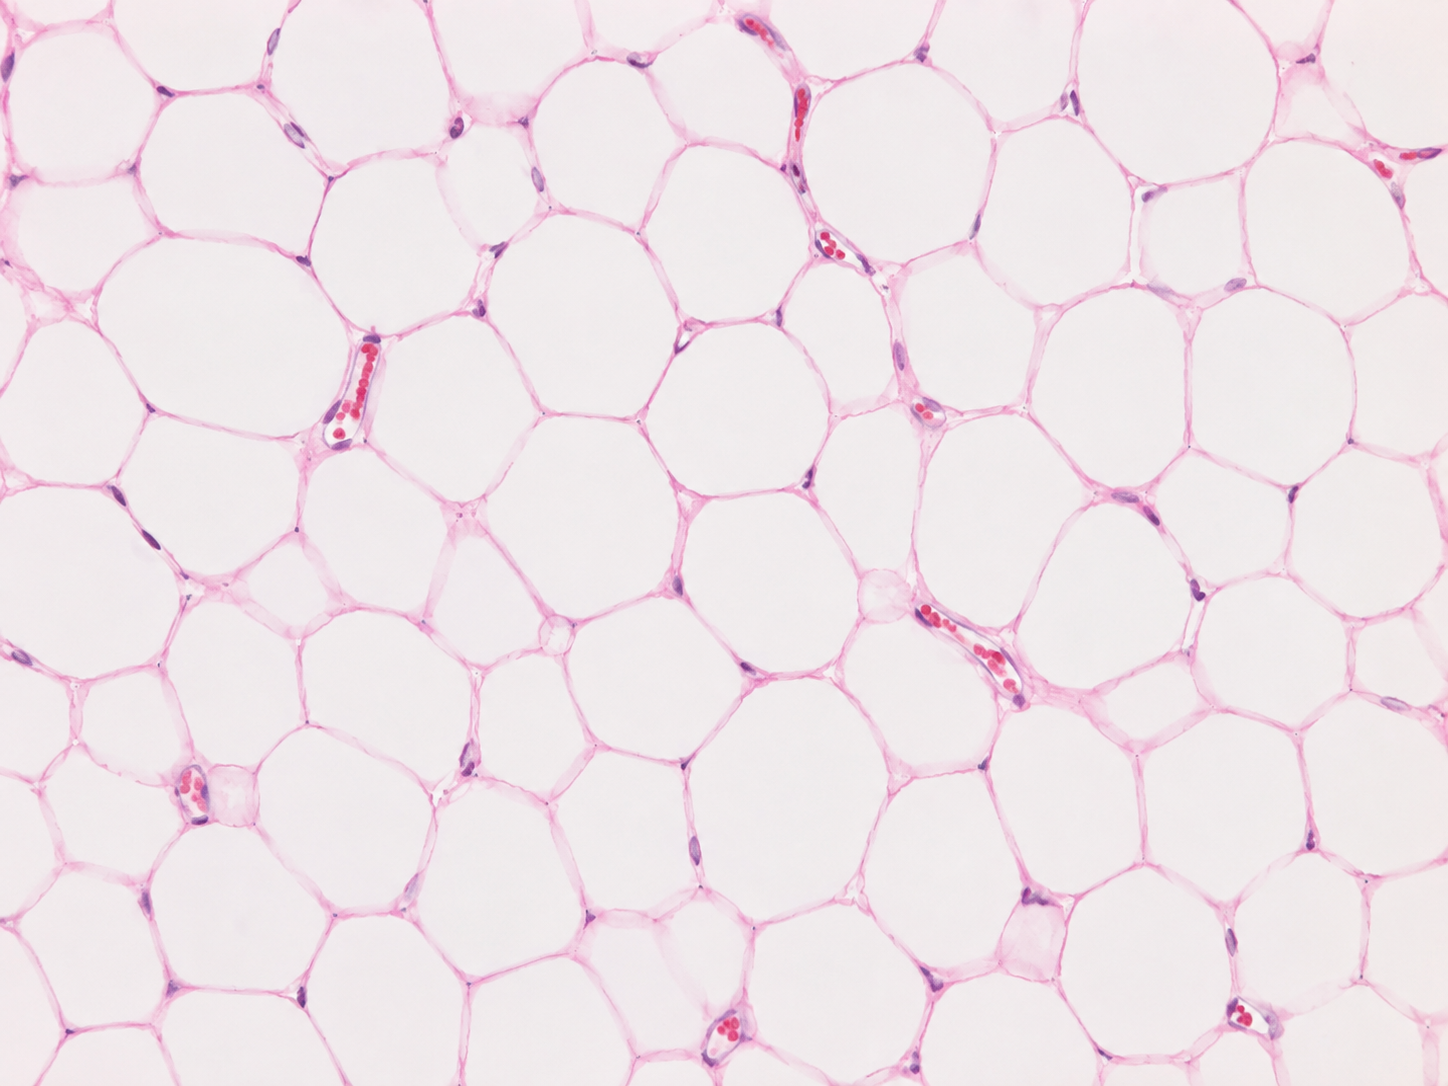
\includegraphics[width=0.5\linewidth]{images/book3/ai/b3-09-adipose-micrograph.png}

{\small \omterm{def:b1:body-plans-tissues:tissue}{Tejido} adiposo blanco: cada \omterm{def:b1:cell-unit-of-life:cell}{célula} es una gota de \omterm{def:b1:lipids:triglyceride}{triglicérido}, de
hasta \qty{100}{\micro m} de diámetro, con su \omterm{def:b1:cell-unit-of-life:cell}{citoplasma} y su núcleo
comprimidos en un reborde delgado. Entre las \omterm{def:b1:cell-unit-of-life:cell}{células} discurren capilares que
entregan y recogen \omterm{def:b1:lipids:fattyacid}{ácidos grasos}.}
\end{omfigure}

\begin{proposition}[La grasa es la reserva de energía más densa]\label{prop:b1:lipids:energystore}
Oxidar \qty{1}{g} de \omterm{def:b1:lipids:triglyceride}{grasa} libera \qty{38}{kJ}, frente a los \qty{17}{kJ} de
\qty{1}{g} de glúcido o de proteína: los carbonos de un \omterm{def:b1:lipids:fattyacid}{ácido graso} están
más reducidos (más enlaces C--H, menos C--O) y por eso ceden más electrones
al oxígeno. Además, la \omterm{def:b1:lipids:triglyceride}{grasa} se almacena seca, mientras que el glucógeno fija
unos \qty{3}{g} de agua por gramo: \qty{1}{g} de glucógeno almacenado rinde
\qty{4}{kJ} por gramo de masa almacenada, y la \omterm{def:b1:lipids:triglyceride}{grasa} nueve veces más. Un ser
humano delgado lleva \qty{0.5}{kg} de glucógeno (la energía de un día) y
\qty{12}{kg} de \omterm{def:b1:lipids:triglyceride}{grasa} (la de más de un mes).
\end{proposition}

\begin{example}[Por qué no almacenarlo todo como grasa]\label{ex:b1:lipids:whyglycogen}
La \omterm{def:b1:lipids:triglyceride}{grasa} solo puede quemarse con oxígeno, despacio, y en los animales no
puede volver a convertirse en glucosa
(\cref{ch:b1:biosyntheses-integration}); el encéfalo y los glóbulos rojos
necesitan glucosa, y un músculo que esprinta la necesita más deprisa de lo
que la \omterm{def:b1:lipids:triglyceride}{grasa} puede suministrarla. El glucógeno es la reserva rápida, sin
oxígeno y de glucosa, para unas horas; la \omterm{def:b1:lipids:triglyceride}{grasa}, la reserva densa para
semanas. Un ave migradora, un lirón que hiberna y un camello son \omterm{def:b1:lipids:triglyceride}{grasa}; las
piernas de un velocista son glucógeno.
\end{example}

\begin{definition}[Ceras]\label{def:b1:lipids:wax}
Las \emph{ceras}\index{cera} son ésteres de un \omterm{def:b1:lipids:fattyacid}{ácido graso} con un alcohol de
cadena larga: sólidas, enteramente hidrófobas y empleadas como recubrimiento
--- la \omterm{def:b1:flowering-plant-organization:tissues}{cutícula} de las \omterm{def:b1:flowering-plant-organization:organs}{hojas}
(\cref{ch:b1:flowering-plant-organization}), la superficie de los insectos,
la impermeabilización de las plumas y del pelaje, el panal de las abejas.
\end{definition}

\section{Lípidos de membrana y autoensamblaje}

\begin{definition}[Lípidos anfífilos]\label{def:b1:lipids:amphiphilic}
Los \omterm{def:b1:lipids:fattyacid}{lípidos} de las membranas son \emph{anfífilos}\index{molécula anfífila}: una \emph{cabeza} \omterm{def:b1:water-small-molecules:water}{polar} que el agua solvata y una o dos
\emph{colas} apolares que excluye. Los
\emph{glicerofosfolípidos}\index{fosfolípido} son glicerol con dos \omterm{def:b1:lipids:fattyacid}{ácidos
grasos} y, en el tercer carbono, un fosfato unido a un alcohol \omterm{def:b1:water-small-molecules:water}{polar} pequeño
(colina, etanolamina, serina, inositol): la fosfatidilcolina es el \omterm{def:b1:lipids:fattyacid}{lípido}
más abundante de las membranas animales. Los
\emph{esfingolípidos}\index{esfingolípido} se construyen sobre el
aminoalcohol esfingosina en vez de sobre glicerol, con un \omterm{def:b1:lipids:fattyacid}{ácido graso} y una
cabeza de fosfocolina (esfingomielina) o de azúcares (glucolípidos), y
abundan en la monocapa externa y en las vainas nerviosas. Los
\emph{esteroles}\index{esterol} --- el \emph{colesterol}\index{colesterol}
en los animales, esteroles emparentados en plantas y hongos --- son
moléculas rígidas de cuatro anillos con un único hidroxilo por cabeza, que
se sitúan entre las colas de los demás \omterm{def:b1:lipids:fattyacid}{lípidos}.
\end{definition}

\begin{proposition}[Autoensamblaje]\label{prop:b1:lipids:selfassembly}
\index{autoensamblaje}\index{micela}\index{liposoma}
En agua, las \omterm{def:b1:lipids:amphiphilic}{moléculas anfífilas} se ensamblan espontáneamente de modo que
esconden sus colas y exponen sus cabezas. La forma de la molécula decide la
estructura: los \omterm{def:b1:lipids:fattyacid}{lípidos} de una sola cola (\omterm{def:b1:lipids:fattyacid}{ácidos grasos}, detergentes), con
forma de cono, forman \emph{micelas} --- esferas de unos nanómetros con las
colas dentro ---; los \omterm{def:b1:lipids:amphiphilic}{fosfolípidos} de dos colas, con forma de cilindro,
forman \emph{bicapas}, que se cierran sobre sí mismas en \emph{liposomas}
(vesículas) para no dejar ningún borde expuesto. El ensamblaje lo impulsa el
\omterm{prop:b1:water-small-molecules:properties}{efecto hidrófobo} (\cref{ch:b1:water-small-molecules}): no cuesta energía ni
necesita enzima, y una bicapa rasgada se vuelve a sellar sola. Las membranas
son láminas que se reparan solas, que crecen por inserción de \omterm{def:b1:lipids:fattyacid}{lípidos} nuevos
y que nunca se forman de la nada: toda membrana procede de una membrana.
\end{proposition}
\begin{proof}[Evidencia]
Un \omterm{def:b1:lipids:amphiphilic}{fosfolípido} seco dispersado en agua forma vesículas cerradas con paredes
en bicapa visibles al \omterm{prop:b1:cell-unit-of-life:microscopes}{microscopio electrónico} (Bangham, 1965); su
permeabilidad a los iones y al agua coincide con la de las membranas
celulares, y pueden cargarse con fármacos y fusionarse con \omterm{def:b1:cell-unit-of-life:cell}{células}. Añadir
un detergente (de una sola cola, con forma de cono) disuelve la bicapa en
micelas mixtas; retirarlo por diálisis deja que la bicapa se rehaga.
\end{proof}

\begin{omfigure}
\begin{tikzpicture}[font=\footnotesize, line cap=round]
  % micelle: ring of heads with tails pointing inward
  \foreach \a in {0,30,...,330} {
    \fill[omDef!60] ({1.2*cos(\a)},{1.2*sin(\a)}) circle (0.14);
    \draw[omDef!70!black, thick] ({1.05*cos(\a)},{1.05*sin(\a)}) -- ({0.35*cos(\a)},{0.35*sin(\a)});
  }
  \node[anchor=north, align=center] at (0,-1.55) {micela: lípidos de\\ una cola (conos)};
  % bilayer segment
  \foreach \i in {0,...,9} {
    \fill[omDef!60] (3.2+0.36*\i,0.75) circle (0.13); \draw[omDef!70!black, thick] (3.14+0.36*\i,0.62) -- (3.14+0.36*\i,0.1) (3.26+0.36*\i,0.62) -- (3.26+0.36*\i,0.1);
    \fill[omDef!60] (3.2+0.36*\i,-0.75) circle (0.13); \draw[omDef!70!black, thick] (3.14+0.36*\i,-0.62) -- (3.14+0.36*\i,-0.1) (3.26+0.36*\i,-0.62) -- (3.26+0.36*\i,-0.1);
  }
  \node[anchor=north, align=center] at (4.85,-1.55) {bicapa: lípidos de\\ dos colas (cilindros)};
  % liposome: two concentric rings of heads with tails between
  \foreach \a in {0,15,...,345} {
    \fill[omDef!60] ({9.3+1.45*cos(\a)},{1.45*sin(\a)}) circle (0.11);
    \draw[omDef!70!black, thick] ({9.3+1.33*cos(\a)},{1.33*sin(\a)}) -- ({9.3+1.0*cos(\a)},{1.0*sin(\a)});
    \fill[omDef!60] ({9.3+0.62*cos(\a)},{0.62*sin(\a)}) circle (0.10);
    \draw[omDef!70!black, thick] ({9.3+0.72*cos(\a)},{0.72*sin(\a)}) -- ({9.3+0.98*cos(\a)},{0.98*sin(\a)});
  }
  \node at (9.3,0) {agua};
  \node[anchor=north, align=center] at (9.3,-1.55) {liposoma: una bicapa\\ cerrada, sin bordes};
\end{tikzpicture}

{\small Tres conjuntos de \omterm{def:b1:lipids:fattyacid}{lípidos} \omterm{def:b1:lipids:amphiphilic}{anfífilos} en agua. Las moléculas de una
sola cola, con forma de cono, se empaquetan en micelas; los \omterm{def:b1:lipids:amphiphilic}{fosfolípidos}
cilíndricos de dos colas forman una bicapa, que se cierra en una vesícula
para esconder sus bordes.}
\end{omfigure}

\begin{omfigure}
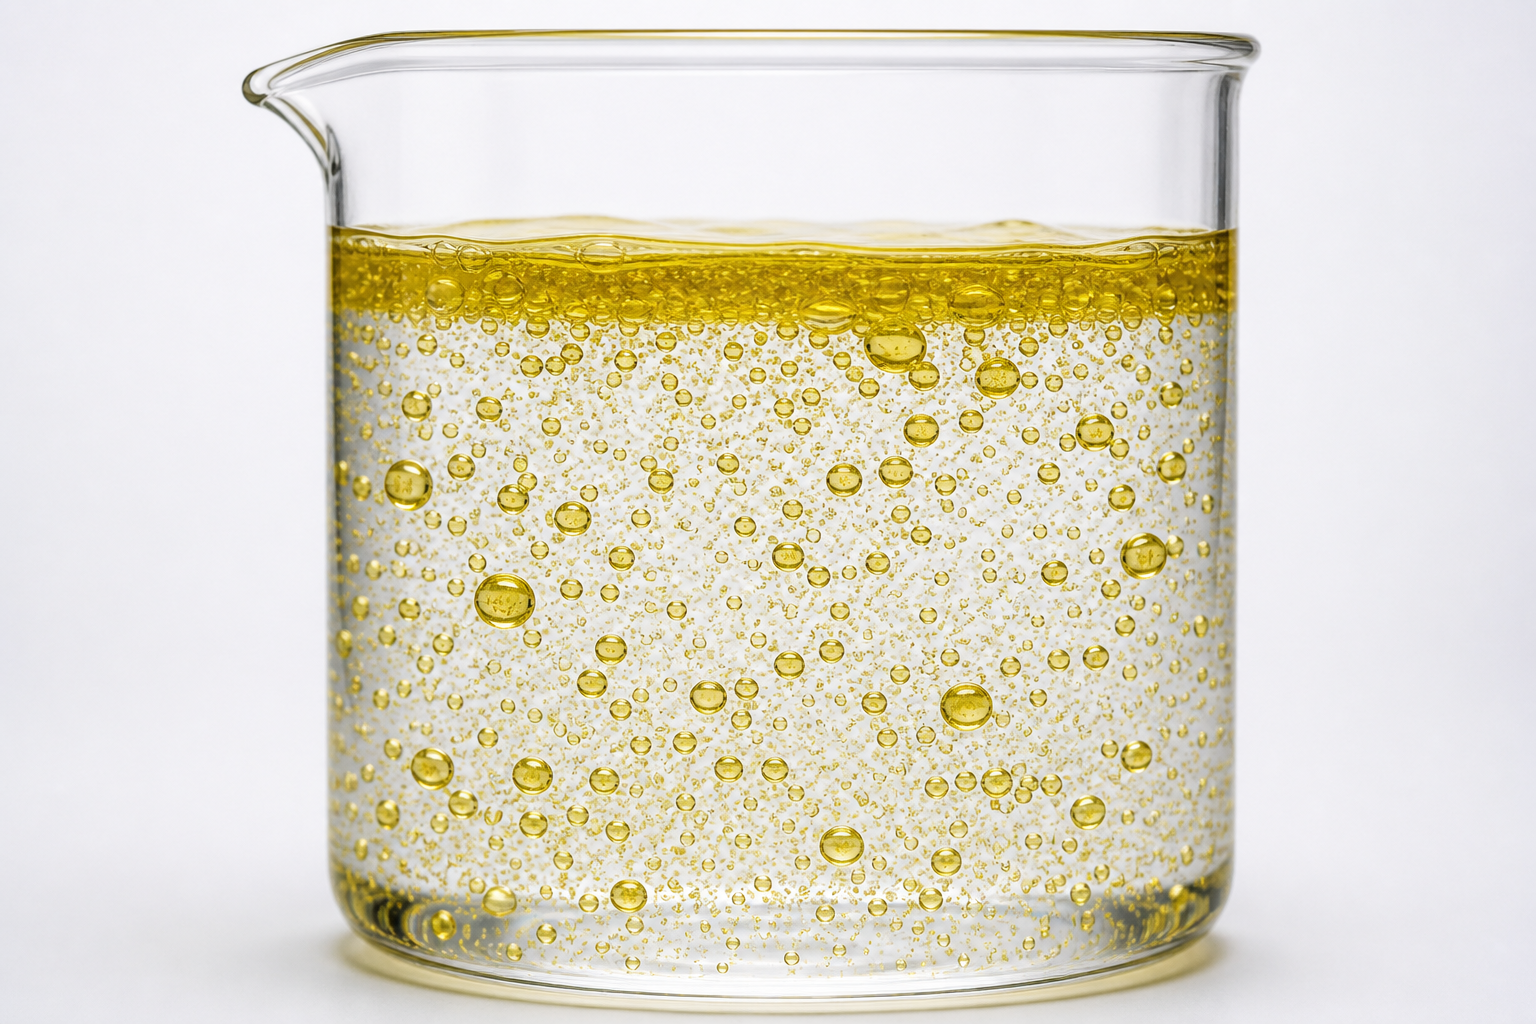
\includegraphics[width=0.5\linewidth]{images/book3/ai/b3-09-oil-water-emulsion.png}

{\small \omterm{def:b1:lipids:triglyceride}{Aceite} agitado en agua: una nube de gotitas que se fusionarán en
minutos, a menos que un anfífilo --- un detergente, una sal biliar, un
\omterm{def:b1:lipids:amphiphilic}{fosfolípido} --- las recubra. La emulsión es lo que el intestino le hace a la
\omterm{def:b1:lipids:triglyceride}{grasa} de la dieta antes de que sus enzimas puedan alcanzarla.}
\end{omfigure}

\begin{example}[Sales biliares]\label{ex:b1:lipids:bile}
La \omterm{def:b1:lipids:triglyceride}{grasa} de la dieta llega al intestino como \omterm{def:b1:lipids:triglyceride}{aceite}; la lipasa que la
digiere solo actúa en la interfase aceite--agua. Las sales biliares,
derivados \omterm{def:b1:lipids:amphiphilic}{anfífilos} del \omterm{def:b1:lipids:amphiphilic}{colesterol}, recubren la \omterm{def:b1:lipids:triglyceride}{grasa} en gotitas de un
micrómetro y multiplican la interfase por mil, y luego llevan los \omterm{def:b1:lipids:fattyacid}{ácidos
grasos} liberados, en micelas, hasta las \omterm{def:b1:cell-unit-of-life:cell}{células} absorbentes
(\cref{ch:b1:digestion-absorption}). El jabón usa el mismo truco.
\end{example}

\section{La fluidez de la membrana}

\begin{definition}[Fluidez, transición de fase]\label{def:b1:lipids:fluidity}
Una \omterm{def:b1:membranes-transport:membrane}{bicapa lipídica} tiene una \emph{temperatura de transición de
fase}\index{temperatura de transición de fase} $T_m$: por debajo de ella las
cadenas están empaquetadas en un estado ordenado, de gel, en el que los
\omterm{def:b1:lipids:fattyacid}{lípidos} apenas se mueven; por encima están desordenadas y la bicapa es un
fluido bidimensional en el que un \omterm{def:b1:lipids:fattyacid}{lípido} cambia de sitio con su vecino un
millón de veces por segundo y recorre el plano de la membrana a
\qty{1}{\micro m/s}. Las \omterm{def:b1:cell-unit-of-life:cell}{células} mantienen sus membranas por encima de
$T_m$: la \emph{fluidez}\index{fluidez de la membrana} permite que las
proteínas difundan y giren, que las vesículas broten y se fusionen y que la
bicapa se vuelva a sellar.
\end{definition}

\begin{proposition}[Qué fija la fluidez]\label{prop:b1:lipids:fluidityfactors}
$T_m$ sube con la longitud de las cadenas y baja con su insaturación, igual
que en los \omterm{def:b1:lipids:fattyacid}{ácidos grasos} libres; una bicapa de cadenas C18:0 funde a
\qty{55}{\celsius} y una de cadenas C18:1, a \qty{-20}{\celsius}. El
\omterm{def:b1:lipids:amphiphilic}{colesterol}, insertado entre las colas, tiene un doble efecto: por encima de
$T_m$ sus anillos rígidos restringen el movimiento de las cadenas y
endurecen la membrana; por debajo de $T_m$ impiden que las cadenas se
empaqueten y evitan que se congele. Ensancha la transición hasta convertirla
en un cambio gradual y mantiene la \omterm{def:b1:lipids:fluidity}{fluidez} casi constante en un amplio
intervalo de temperatura: es un \omterm{def:b1:water-small-molecules:buffer}{tampón} de \omterm{def:b1:lipids:fluidity}{fluidez}. Las membranas plasmáticas
animales llegan a tener un \omterm{def:b1:lipids:amphiphilic}{colesterol} por cada \omterm{def:b1:lipids:amphiphilic}{fosfolípido}.
\end{proposition}

\begin{omfigure}
\begin{tikzpicture}
\begin{axis}[
  width=0.86\linewidth, height=6.0cm,
  axis x line=bottom, axis y line=left,
  xmin=-20, xmax=60, ymin=0, ymax=1.15,
  xlabel={temperatura (\unit{\celsius})}, ylabel={fluidez (relativa)},
  xlabel style={font=\small, at={(axis description cs:0.5,-0.12)}, anchor=north},
  ylabel style={font=\small},
  tick label style={font=\small}, xtick={-20,0,20,40,60}, ytick={0,0.5,1},
  legend style={font=\small, at={(0.03,0.97)}, anchor=north west, draw=none},
  clip=false,
]
\addplot[very thick, omDef, domain=-20:60, samples=120] {1/(1+exp(-(x-41)/1.5))};
\addlegendentry{cadenas C16 saturadas, sin colesterol}
\addplot[very thick, omProp, domain=-20:60, samples=120] {1/(1+exp(-(x+5)/1.5))};
\addlegendentry{un doble enlace \emph{cis} por lípido}
\addplot[very thick, omThm, domain=-20:60, samples=120] {0.15+0.7/(1+exp(-(x-20)/12))};
\addlegendentry{cadenas saturadas con \qty{30}{\%} de colesterol}
\draw[dashed, gray] (axis cs:37,0) -- (axis cs:37,1.05);
\node[font=\scriptsize, anchor=south] at (axis cs:37,1.06) {\qty{37}{\celsius}};
\end{axis}
\end{tikzpicture}

{\small \omterm{def:b1:lipids:fluidity}{Fluidez} frente a temperatura para tres bicapas. Las cadenas
saturadas se congelan bruscamente cerca de \qty{40}{\celsius}; un doble
enlace por \omterm{def:b1:lipids:fattyacid}{lípido} baja la transición por debajo de cero; el \omterm{def:b1:lipids:amphiphilic}{colesterol}
suaviza la transición hasta una pendiente leve y mantiene la membrana ni
sólida ni demasiado fluida en todo el intervalo fisiológico.}
\end{omfigure}

\begin{proposition}[Adaptación homeoviscosa]\label{prop:b1:lipids:homeoviscous}
\index{adaptación homeoviscosa}
Los \omterm{def:b1:organism-environment:organism}{organismos} que no pueden regular su temperatura ajustan la composición
de sus membranas para mantener constante la \omterm{def:b1:lipids:fluidity}{fluidez}: cuando la temperatura
baja, sustituyen \omterm{def:b1:lipids:fattyacid}{ácidos grasos saturados} por \omterm{def:b1:lipids:fattyacid}{insaturados} y cadenas largas
por otras más cortas, y al revés cuando sube.
\end{proposition}
\begin{proof}[Evidencia]
\emph{E. coli} cultivada a \qty{10}{\celsius} tiene el doble de proporción
de \omterm{def:b1:lipids:fattyacid}{ácidos grasos insaturados} que la misma cepa cultivada a
\qty{40}{\celsius}, y las membranas de ambos cultivos, medidas por la
movilidad de una sonda, son igual de fluidas a sus temperaturas de
cultivo. Las truchas aclimatadas a \qty{5}{\celsius} llevan más ácidos
poliinsaturados en los \omterm{def:b1:lipids:fattyacid}{lípidos} de sus membranas que las truchas a
\qty{20}{\celsius}; la \omterm{def:b1:lipids:triglyceride}{grasa} de las patas de un reno, junto a la nieve, es
más insaturada que la del tronco. Las plantas que sobreviven a las heladas
enriquecen sus membranas en \omterm{def:b1:lipids:fattyacid}{lípidos} \omterm{def:b1:lipids:fattyacid}{insaturados} en otoño, y los mutantes
incapaces de hacerlo mueren al enfriarse.
\end{proof}

\begin{example}[Mantequilla, aceite de oliva, aceite de pescado]\label{ex:b1:lipids:kitchen}
La mantequilla (\qty{65}{\%} saturada) es sólida en el frigorífico y blanda
a temperatura ambiente; el \omterm{def:b1:lipids:triglyceride}{aceite} de oliva (\qty{75}{\%} de ácido oleico) es
líquido a temperatura ambiente y se enturbia en el frigorífico; el \omterm{def:b1:lipids:triglyceride}{aceite} de
pescado, rico en ácidos omega-3 con cinco y seis dobles enlaces, sigue
líquido a \qty{-20}{\celsius}, que es lo que necesitan las membranas de un
bacalao en el Atlántico Norte.
\end{example}

\section{Esteroles, pigmentos y señales}

\begin{definition}[Esteroides, isoprenoides]\label{def:b1:lipids:steroids}
Los \emph{esteroides}\index{esteroide} comparten los cuatro anillos
condensados del \omterm{def:b1:lipids:amphiphilic}{colesterol}: el propio \omterm{def:b1:lipids:amphiphilic}{colesterol} (membranas, y precursor de
todos los demás), las sales biliares, la vitamina D y las hormonas
esteroideas --- cortisol, aldosterona, hormonas sexuales ---, moléculas
pequeñas e hidrófobas que atraviesan libremente las membranas y actúan sobre
receptores del interior de la \omterm{def:b1:cell-unit-of-life:cell}{célula}. Los
\emph{isoprenoides}\index{isoprenoide} (terpenos) son cadenas y anillos de
unidades de isopreno de cinco carbonos: los \emph{carotenoides} que dan
color a las zanahorias y protegen los \omterm{def:b1:eukaryotic-cell:plastid}{cloroplastos}
(\cref{ch:b1:photosynthesis}), la cadena lateral de la clorofila, las
quinonas de las cadenas de transporte de electrones, el caucho y las
vitaminas liposolubles A, E y K.
\end{definition}

\begin{proposition}[Lo que hacen los lípidos]\label{prop:b1:lipids:functions}
Almacenar energía (\omterm{def:b1:lipids:triglyceride}{triglicéridos}); formar membranas (\omterm{def:b1:lipids:amphiphilic}{fosfolípidos},
\omterm{def:b1:lipids:amphiphilic}{esfingolípidos}, \omterm{def:b1:lipids:amphiphilic}{esteroles}); aislar e impermeabilizar (\omterm{def:b1:lipids:triglyceride}{grasa}, \omterm{def:b1:lipids:wax}{ceras}); captar
luz y proteger (carotenoides); transportar electrones (quinonas); señalizar
entre \omterm{def:b1:cell-unit-of-life:cell}{células} (hormonas esteroideas, prostaglandinas) y dentro de ellas
(\omterm{def:b1:lipids:amphiphilic}{fosfolípidos} de inositol, diacilglicerol); actuar como vitaminas. Una sola
propiedad --- la insolubilidad en agua --- subyace a todas ellas: un \omterm{def:b1:lipids:fattyacid}{lípido}
se queda donde se le pone, en una gota, una película o una membrana, o
atraviesa una membrana sin \omterm{def:b1:membranes-transport:transporters}{transportador}.
\end{proposition}

\begin{example}[Una hormona que no necesita receptor en la superficie]\label{ex:b1:lipids:steroidhormone}
El cortisol, secretado por la glándula suprarrenal, viaja por la sangre
unido a una proteína transportadora, la abandona al llegar a una \omterm{def:b1:cell-unit-of-life:cell}{célula}
diana, se disuelve a través de la membrana plasmática en segundos y se une a
un receptor del \omterm{def:b1:eukaryotic-cell:organelle}{citosol} que entra después en el núcleo y activa genes
(\cref{ch:b1:expression-control}). Una hormona proteica como la insulina,
hidrosoluble y demasiado grande para atravesarla, debe unirse a un receptor
del exterior y hacer que su mensaje se transmita hacia dentro. La química
del mensajero decide la ruta del mensaje.
\end{example}

\section{Ejercicios}

\begin{exercise}[$\star$]\label{exo:b1:lipids:1}
Defínase un \omterm{def:b1:lipids:fattyacid}{lípido} y explíquese por qué la definición es por una propiedad y
no por una estructura.
\end{exercise}

\begin{exercise}[$\star$]\label{exo:b1:lipids:2}
Escríbase la notación del ácido linoleico (18 carbonos, dobles enlaces tras
los carbonos 9 y 12) y dígase si es un ácido omega-3 u omega-6.
\end{exercise}

\begin{exercise}[$\star$]\label{exo:b1:lipids:3}
¿Por qué un \omterm{def:b1:lipids:triglyceride}{triglicérido} forma gotas y un \omterm{def:b1:lipids:amphiphilic}{fosfolípido} forma bicapas? ¿Qué
diferencia estructural lo explica?
\end{exercise}

\begin{exercise}[$\star$]\label{exo:b1:lipids:4}
A partir de la figura de la \omterm{def:b1:lipids:fluidity}{fluidez}, ¿a qué temperatura está cada una de las
tres bicapas a mitad de su transición? ¿Cuál cabría esperar en una bacteria
que vive a \qty{10}{\celsius}?
\end{exercise}

\begin{exercise}[$\star\star$]\label{exo:b1:lipids:5}
Una persona almacena \qty{15}{kg} de \omterm{def:b1:lipids:triglyceride}{grasa}. Calcúlense la energía que
contiene, el número de días que sostendría un gasto en reposo de
\qty{8}{MJ/d} y la masa de glucógeno hidratado que contendría esa misma
energía.
\end{exercise}

\begin{exercise}[$\star\star$]\label{exo:b1:lipids:6}
Ordénense por punto de fusión: C14:0, C18:0, C18:1, C18:3, C22:0, y
justifíquese cada paso de la ordenación.
\end{exercise}

\begin{exercise}[$\star\star$]\label{exo:b1:lipids:7}
Un glóbulo rojo tiene una superficie de \qty{140}{\micro m^2}; una cabeza de
\omterm{def:b1:lipids:amphiphilic}{fosfolípido} ocupa \qty{0.6}{nm^2}. Calcúlense el número de moléculas de
\omterm{def:b1:lipids:amphiphilic}{fosfolípido} de la membrana (dos monocapas) y, a \qty{750}{g/mol}, su masa
total en picogramos.
\end{exercise}

\begin{exercise}[$\star\star$]\label{exo:b1:lipids:8}
Se emulsiona \qty{1}{g} de \omterm{def:b1:lipids:triglyceride}{aceite} de oliva (densidad \qty{0.9}{g/mL}) en
gotitas de \qty{1}{\micro m} de diámetro. Calcúlese el área total de la
interfase. Repítase para una sola gota. ¿Por qué necesita la lipasa
pancreática la emulsión?
\end{exercise}

\begin{exercise}[$\star\star$]\label{exo:b1:lipids:9}
Explíquense los dos efectos opuestos del \omterm{def:b1:lipids:amphiphilic}{colesterol} sobre la \omterm{def:b1:lipids:fluidity}{fluidez de la
membrana} y por qué una membrana con \omterm{def:b1:lipids:amphiphilic}{colesterol} no tiene una transición
brusca.
\end{exercise}

\begin{exercise}[$\star\star\star$]\label{exo:b1:lipids:10}
Una planta mutante no puede fabricar \omterm{def:b1:lipids:fattyacid}{ácidos grasos insaturados}. Predíganse
sus membranas a \qty{25}{\celsius} y a \qty{5}{\celsius}, qué les ocurre a
sus \omterm{def:b1:cell-unit-of-life:cell}{células} en una noche fría y por qué sobrevive la planta silvestre.
\end{exercise}

\begin{exercise}[$\star\star\star$]\label{exo:b1:lipids:11}
La \omterm{def:b1:lipids:triglyceride}{grasa} da \qty{1.07}{g} de agua por gramo oxidado (el glucógeno
\qty{0.56}{g} y la proteína \qty{0.4}{g}). Calcúlese el agua producida por
un camello que oxida \qty{1}{kg} de \omterm{def:b1:lipids:triglyceride}{grasa}. El oxígeno necesario es de
\qty{2}{L} por gramo de \omterm{def:b1:lipids:triglyceride}{grasa}; respirarlo en el aire seco del desierto
cuesta unos \qty{0.03}{g} de agua por litro de aire ventilado, con una
extracción de oxígeno del \qty{5}{\%}. Calcúlese el agua perdida al respirar
y dígase si la joroba es una reserva de agua.
\end{exercise}

\begin{exercise}[$\star\star\star$]\label{exo:b1:lipids:12}
``Una membrana se ensambla sola, pero una \omterm{def:b1:cell-unit-of-life:cell}{célula} no puede fabricar una
membrana de la nada.'' Concíliense las dos mitades de la frase en un
párrafo, usando el \omterm{prop:b1:water-small-molecules:properties}{efecto hidrófobo}, el crecimiento de las membranas por
inserción y la continuidad de las membranas a lo largo de la división
celular.
\end{exercise}

\section{Problema: agua fría y grasa del desierto}

\begin{problem}[{Problema de fin de semana --- las membranas de una trucha
en un arroyo de montaña y la joroba de un camello en el desierto:
insaturación, temperaturas de transición, densidad energética y agua
metabólica, hasta llegar a la masa que ahorra almacenar grasa en vez de
glucógeno}]
\label{pb:b1:lipids:1}
La parte I trata de una trucha cuyos \omterm{def:b1:lipids:amphiphilic}{fosfolípidos} de membrana llevan cadenas
C16:0, C18:1 y C22:6 (un ácido omega-3 con seis dobles enlaces). La parte II
trata de un dromedario de \qty{500}{kg} con una joroba de \qty{30}{kg} de
\omterm{def:b1:lipids:triglyceride}{triglicérido}, que cruza un desierto con una \omterm{def:b1:organism-environment:allometry}{tasa metabólica} de
\qty{60}{MJ/d}. Energía: \omterm{def:b1:lipids:triglyceride}{grasa} \qty{38}{kJ/g}, glucógeno \qty{17}{kJ/g} en
seco, almacenado con \qty{3}{g} de agua por gramo. Agua metabólica:
\qty{1.07}{g/g} de \omterm{def:b1:lipids:triglyceride}{grasa}. Oxígeno: \qty{2.0}{L} por gramo de \omterm{def:b1:lipids:triglyceride}{grasa}; el aire
tiene un \qty{21}{\%} de oxígeno; el camello extrae el \qty{5}{\%} del
oxígeno que respira; el aire exhalado lleva \qty{30}{g/m^3} de agua más que
el aire del desierto inhalado.

\medskip
\noindent\textbf{Parte I --- La trucha.}
Las truchas aclimatadas a \qty{20}{\celsius} tienen cadenas de membrana con
un \qty{40}{\%} de C16:0, un \qty{45}{\%} de C18:1 y un \qty{15}{\%} de
C22:6; las truchas a \qty{5}{\celsius}, un \qty{25}{\%}, un \qty{40}{\%} y
un \qty{35}{\%}.
\begin{enumerate}
  \item Escríbase la notación de los tres ácidos y cuéntense los dobles
        enlaces por cadena en cada uno.
  \item Calcúlese el número medio de dobles enlaces por cadena a cada
        temperatura.
  \item Explíquese, a partir del empaquetamiento de las cadenas, por qué el
        cambio rebaja la temperatura de transición de la membrana.
  \item La $T_m$ de una bicapa baja unos \qty{20}{\celsius} por cada
        \qty{0.5}{} dobles enlaces más por cadena en promedio. Estímese el
        desplazamiento de $T_m$ entre las dos truchas.
  \item La membrana de la trucha de aguas cálidas es fluida a
        \qty{20}{\celsius}, pero gelificaría a \qty{5}{\celsius}. ¿Qué les
        ocurriría a sus proteínas de transporte, a sus \omterm{def:b1:membranes-transport:transporters}{bombas} y a su
        conducción nerviosa en una noche fría repentina?
  \item La adaptación tarda días. Nómbrense las enzimas que la trucha debe
        fabricar en mayor cantidad, y dónde actúan en la \omterm{def:b1:cell-unit-of-life:cell}{célula}
        (\cref{ch:b1:eukaryotic-cell}).
  \item El \omterm{def:b1:lipids:amphiphilic}{colesterol} está a razón de una molécula por cada dos
        \omterm{def:b1:lipids:amphiphilic}{fosfolípidos} en las dos truchas. Explíquese qué aporta en cada
        caso.
\end{enumerate}

\medskip
\noindent\textbf{Parte II --- La energía del camello.}
\begin{enumerate}[resume]
  \item Calcúlese la energía almacenada en la joroba.
  \item ¿Para cuántos días de travesía basta?
  \item Calcúlense la masa de glucógeno seco que contiene esa misma energía
        y la masa de glucógeno hidratado.
  \item Calcúlese la masa ahorrada al almacenar \omterm{def:b1:lipids:triglyceride}{grasa} en vez de glucógeno,
        y exprésese como fracción de la masa corporal del camello.
  \item La \omterm{def:b1:lipids:triglyceride}{grasa} se almacena en una joroba y no repartida bajo la piel.
        Propóngase una razón, a partir del balance térmico del
        \cref{ch:b1:mammal-organization}.
\end{enumerate}

\medskip
\noindent\textbf{Parte III --- ¿Es la joroba una reserva de agua?}
\begin{enumerate}[resume]
  \item Calcúlese el agua metabólica producida al oxidar toda la joroba.
  \item Calcúlese el oxígeno necesario, en litros.
  \item Calcúlese el volumen de aire que el camello debe ventilar para
        obtenerlo.
  \item Calcúlese el agua perdida al exhalar ese aire.
  \item Compárese el agua ganada con el agua perdida y conclúyase.
  \item En vez de sudar, el camello deja subir su temperatura corporal
        \qty{6}{\celsius} durante el día y se enfría de noche. Calcúlense
        el calor que almacena así (capacidad calorífica
        \qty{3.5}{kJ.kg^{-1}.K^{-1}}) y el agua que costaría evaporar ese
        mismo calor (\qty{2.4}{kJ/g}).
  \item Un camello puede perder el \qty{25}{\%} de su agua corporal y
        sobrevivir, y sus glóbulos rojos se hinchan hasta el doble de su
        volumen sin reventar cuando bebe \qty{100}{L} en diez minutos.
        Relaciónese la segunda propiedad con las membranas del
        \cref{ch:b1:membranes-transport}.
\end{enumerate}

\medskip
\noindent\textbf{Parte IV --- La aritmética de la bicapa.}
Una cabeza de \omterm{def:b1:lipids:amphiphilic}{fosfolípido} ocupa \qty{0.65}{nm^2}; una bicapa tiene
\qty{5}{nm} de espesor; los glóbulos rojos del camello tienen una superficie
de \qty{80}{\micro m^2} y son $\num{8e12}$ por litro de sangre.
\begin{enumerate}[resume]
  \item Calcúlese el número de \omterm{def:b1:lipids:amphiphilic}{fosfolípidos} de la membrana de un glóbulo
        rojo.
  \item Calcúlese el número de todos los glóbulos rojos de \qty{40}{L} de
        sangre.
  \item A \qty{750}{g/mol}, calcúlese la masa de ese \omterm{def:b1:lipids:fattyacid}{lípido} en gramos.
  \item Un \omterm{def:b1:lipids:amphiphilic}{fosfolípido} pasa espontáneamente de una monocapa a la otra
        aproximadamente una vez por semana, pero difunde lateralmente
        \qty{1}{\micro m} en un segundo. Explíquense ambas cifras a partir
        del \omterm{prop:b1:water-small-molecules:properties}{efecto hidrófobo}.
  \item Explíquese por qué, dada esa frecuencia de volteo, las dos
        monocapas de una membrana pueden mantener composiciones distintas
        durante toda la vida de una \omterm{def:b1:cell-unit-of-life:cell}{célula}.
  \item Enúnciese el resultado: la masa que ahorra el camello al llevar
        \qty{30}{kg} de \omterm{def:b1:lipids:triglyceride}{grasa} en vez del glucógeno de igual energía, y el
        veredicto sobre la joroba como reserva de agua.
\end{enumerate}
\end{problem}
